\chapter{Desenvolvimento do Ambiente Experimental}
\label{cap:desenvolvimento}

\section{Visão geral do ambiente experimental}
\label{sec:visao_geral_ambiente}
\label{subsec:adequacao_tipo_projeto}

O produto deste trabalho é um ambiente laboratorial controlado, e não um sistema de informação: não há aplicação, banco de dados ou interface própria, e por isso não foram elaborados diagramas de classes, de sequência ou modelos entidade-relacionamento. A documentação do desenvolvimento concentra-se na configuração da rede, na integração dos componentes, na organização das evidências e nos critérios de validação, representados por um diagrama de blocos (arquitetura) e um fluxograma (sequência dos ensaios).

O ambiente foi composto por um ponto de acesso Wi-Fi, uma plataforma de ataque LILYGO T-Embed CC1101 Plus (ESP32-S3, \textit{firmware} Bruce 1.16.1), três dispositivos IoT comerciais, um \textit{smartphone} de referência e uma estação de captura formada por um \textit{notebook} com Kali Linux em máquina virtual e um adaptador Wi-Fi em modo monitor. Esse conjunto foi usado para executar os ensaios de desautenticação, registrar os quadros IEEE~802.11 e medir o tempo sem resposta de cada dispositivo. O ponto de acesso foi operado em duas configurações de segurança (WPA2 e modo misto WPA2/WPA3), e a segurança efetivamente negociada por cada dispositivo foi verificada nos quadros de associação (Apêndice~\ref{sec:evidencias-rsn}).

\section{Requisitos e regras experimentais}
\label{sec:requisitos_experimento}

Os requisitos foram definidos a partir da fundamentação sobre quadros de gerenciamento do IEEE~802.11 \cite{KohliosHayajneh2018,Amoordon2022}, das características das plataformas ESP \cite{LitayemAlsadi2023} e dos procedimentos da metodologia. Para cada requisito, indica-se como foi atendido.

\subsection{Requisitos funcionais}
\label{subsec:requisitos_funcionais}

\begin{itemize}
    \item \textbf{RF01 --- Configuração dos cenários de segurança:} o ponto de acesso foi operado em WPA2-PSK[AES] e em modo misto WPA2-PSK[AES]+WPA3-\textit{Personal}, com o estado de PMF registrado a partir dos \textit{beacons} (Seção~\ref{sec:configuracao_rede_teste}).
    \item \textbf{RF02 --- Associação dos dispositivos:} câmera, lâmpada, tomada e \textit{smartphone} foram associados à rede TCC\_LAB, criada exclusivamente para o experimento.
    \item \textbf{RF03 --- Preparação da plataforma de ataque:} o \textit{firmware} Bruce 1.16.1 foi instalado no T-Embed CC1101 Plus e sua função de desautenticação foi validada no ensaio piloto.
    \item \textbf{RF04 --- Captura de tráfego IEEE~802.11:} o adaptador AR9271 foi colocado em modo monitor no canal 6 e gravou arquivos \texttt{.pcapng} legíveis em todos os ensaios.
    \item \textbf{RF05 --- Registro de conectividade:} cada ensaio, exceto o piloto, teve um \textit{log} de \textit{ping} com marcas de tempo, iniciado junto com a captura.
    \item \textbf{RF06 --- Repetição:} previstas três repetições por combinação; atendido no cenário WPA2 para tomada, lâmpada e \textit{smartphone}, e não atendido para a câmera e para o modo misto (ver Seção~\ref{sec:limitacoes_ambiente}).
\end{itemize}

\subsection{Requisitos não funcionais}
\label{subsec:requisitos_nao_funcionais}

\begin{itemize}
    \item \textbf{RNF01 --- Uso ético e controlado:} os testes ocorreram apenas na rede própria, sem interferência intencional em redes ou usuários de terceiros.
    \item \textbf{RNF02 --- Proteção de informações sensíveis:} senhas foram omitidas das figuras; credenciais e conteúdos privados não foram divulgados.
    \item \textbf{RNF03 --- Rastreabilidade:} modelos, versões, canal, segurança e PMF foram registrados (Seções~\ref{sec:configuracao_rede_teste} e~\ref{sec:inventario}).
    \item \textbf{RNF04 --- Comparabilidade:} as condições físicas e operacionais entre repetições estão descritas na Seção~\ref{sec:condicoes_experimentais}.
    \item \textbf{RNF05 --- Evidências verificáveis:} cada ensaio gerou um arquivo de captura e, exceto o piloto, um \textit{log} de \textit{ping}, preservados com nomes que identificam dispositivo, cenário e repetição.
\end{itemize}

\subsection{Regras experimentais}
\label{sec:regras_experimentais}

\begin{itemize}
    \item \textbf{RE01 --- Delimitação da rede:} todas as execuções ocorreram somente na rede de laboratório.
    \item \textbf{RE02 --- Dispositivos avaliados:} câmera, lâmpada e tomada foram mantidos nas duas configurações; o \textit{smartphone} serviu como referência.
    \item \textbf{RE03 --- Critério de conectividade:} a conectividade foi verificada por \textit{ping} ao endereço IP de cada dispositivo; no ensaio piloto, sem \textit{ping}, usou-se a presença de quadros de dados da câmera na captura.
    \item \textbf{RE04 --- Escopo:} apenas o ataque de desautenticação foi executado; o \textit{Evil Twin} foi tratado somente no referencial teórico.
\end{itemize}

\section{Configuração da rede de teste}
\label{sec:configuracao_rede_teste}

A rede de teste TCC\_LAB foi criada no roteador TP-Link EX1500, na faixa de 2,4~GHz, canal 6 (2437~MHz), com largura de 20~MHz. Para que o \textit{smartphone}, inicialmente associado em 5~GHz, pudesse ser avaliado, a direção de banda (\textit{band steering}) foi desabilitada, forçando-o a 2,4~GHz. Foram utilizadas duas configurações de segurança:

\begin{itemize}
    \item \textbf{WPA2:} WPA2-PSK[AES]. O painel não apresentou PMF habilitado nesse modo, e os \textit{beacons} capturados anunciam somente o AKM~2 (PSK), com MFPC~=~0, ou seja, o ponto de acesso não ofereceu PMF;
    \item \textbf{Modo misto:} WPA2-PSK[AES]+WPA3-\textit{Personal}. Os \textit{beacons} anunciam os AKM~2 (PSK) e~8 (SAE), com MFPC~=~1 e MFPR~=~0, isto é, PMF oferecido de forma opcional.
\end{itemize}

Não foi executada uma condição de WPA2 com PMF nem de WPA3 exclusivo; esta última porque câmera e tomada não se associam a uma rede somente WPA3. Os valores dos \textit{beacons} e a segurança negociada por dispositivo constam do Apêndice~\ref{sec:evidencias-rsn}.

\section{Inventário de equipamentos e ferramentas}
\label{sec:inventario}
\label{sec:equipamentos_ferramentas}

O Quadro~\ref{quad:inventario} reúne os equipamentos e as versões de \textit{software} empregados. Todos os campos foram obtidos dos próprios equipamentos e da documentação dos fabricantes; nenhum foi estimado.

\begin{quadro}[htbp]
\centering
\caption{Inventário de equipamentos e ferramentas}
\label{quad:inventario}
\marcadoresTabela
\small
\renewcommand{\arraystretch}{1.15}
\begin{tabular}{|>{\raggedright\arraybackslash}p{0.23\textwidth}|>{\raggedright\arraybackslash}p{0.70\textwidth}|}
\hline
\textbf{Item} & \textbf{Identificação e versão} \\ \hline
Ponto de acesso & TP-Link EX1500; \textit{firmware} 1.13.0; revisão de \textit{hardware} V1 \\ \hline
Plataforma de ataque & LILYGO T-Embed CC1101 Plus, SoC ESP32-S3 \cite{LilygoTEmbed,EspressifS3Datasheet}; \textit{firmware} Bruce 1.16.1 \cite{BruceFirmware} \\ \hline
Câmera IP & Xiaomi, nome comercial Mi 360 PTZ 2K (nome de rede \texttt{chuangmi\_camera\_029a02}); código de modelo PTZ 2K; \textit{firmware} 4.3.4\_0425 \\ \hline
Lâmpada inteligente & Marca de revenda ``Guillermo'' (sem fabricante próprio identificado); modelo \texttt{Smart Wifi Light Bulb} (base E27, 9~W, RGB + branco, aplicativo CozyLife, 2,4~GHz); \textit{firmware} 1.0.12 \\ \hline
Tomada inteligente & Marca TNCE; modelo \texttt{Smart Brazil Plug} (padrão brasileiro 16/20~A, Wi-Fi 2,4~GHz, aplicativo Smart Life/Tuya, com medição de energia); \textit{firmware} 1.0.2 \\ \hline
\textit{Smartphone} de referência & Samsung Galaxy S21; Android 15; One UI 7.0; endereço MAC aleatório por rede (bit de administração local ativo no endereço observado) \\ \hline
Adaptador de captura & Qualcomm Atheros AR9271 (USB 0cf3:9271), \textit{driver} ath9k\_htc, modo monitor \cite{Ath9kHtc} \\ \hline
Virtualização & Oracle VirtualBox 7.2.6 (versão instalada no hospedeiro na data da redação); adaptador USB repassado à máquina virtual \\ \hline
Sistema de captura & Kali Linux 2026.2; \textit{tcpdump} 4.99.6; Wireshark 4.6.6 (ensaio piloto) \\ \hline
Ferramenta de análise & \textit{tshark} 4.6.4 (Windows), sobre arquivos com encapsulamento IEEE~802.11 + Radiotap \\ \hline
\end{tabular}
\legend{Fonte: elaborado pelo autor com base na documentação dos fabricantes e nos registros do ensaio (2026).}
\end{quadro}

Conforme o Quadro~\ref{quad:inventario}, a plataforma de ataque reúne, na mesma placa, o SoC ESP32-S3 e um transceptor CC1101. Os quadros de desautenticação foram transmitidos exclusivamente pelo rádio Wi-Fi do ESP32-S3, que opera em IEEE~802.11 b/g/n na faixa de 2,4~GHz \cite{EspressifS3Datasheet}. O CC1101 é um transceptor para faixas abaixo de 1~GHz, que não opera em Wi-Fi e não foi utilizado nos ensaios; ele apenas dá nome à placa.

\section{Condições experimentais}
\label{sec:condicoes_experimentais}

O Quadro~\ref{quad:condicoes} registra as condições sob as quais os ensaios foram realizados. As condições foram obtidas dos próprios arquivos de captura e dos registros do pesquisador.

\begin{quadro}[htbp]
\centering
\caption{Condições de execução dos ensaios}
\label{quad:condicoes}
\marcadoresTabela
\small
\renewcommand{\arraystretch}{1.15}
\begin{tabular}{|>{\raggedright\arraybackslash}p{0.27\textwidth}|>{\raggedright\arraybackslash}p{0.66\textwidth}|}
\hline
\textbf{Condição} & \textbf{Registro} \\ \hline
Datas & Ensaio piloto da câmera: 3 nov. 2026; demais ensaios: 8 nov. 2026; em 17 nov. 2026, das 19:05 às 20:04, seis capturas da câmera em WPA2: \texttt{R03} e \texttt{R04}, válidas com \textit{ping}; \texttt{R05} e \texttt{R06}, invalidadas; \texttt{R07}, teste de bancada; \texttt{R08}, descritiva (Apêndice~\ref{sec:registro-execucoes}; marcas de tempo dos arquivos de captura) \\ \hline
Canal e largura & Canal 6 (2437~MHz), 20~MHz, em todos os ensaios \\ \hline
Duração das capturas & Ensaios de ataque: 79 a 254,9~s; captura dedicada da lâmpada: 64,0~s; as execuções \texttt{CAM\_WPA2\_R03} e \texttt{CAM\_WPA2\_R04} duraram 254,9~s e 215,0~s, respectivamente (Tabelas~\ref{tab:registro-execucoes} e~\ref{tab:registro-metricas}, Apêndice~\ref{sec:registro-execucoes}) \\ \hline
Janelas de referência, ataque e pós-ataque & Referência: linha de base com respostas normais ao \textit{ping} antes do primeiro quadro de desautenticação direcionado ao dispositivo; duração planejada de 20 a 30~s e, nas execuções válidas, de cerca de 8,5~s a 105~s. Ataque: duração planejada de 20 a 30~s; na prática, o ataque foi encerrado manualmente e durou de cerca de 18~s a 120~s. Pós-ataque: duração planejada de 20 a 30~s. Instantes de início e fim do ataque por execução: Tabelas~\ref{tab:registro-execucoes} e~\ref{tab:registro-metricas} \\ \hline
Distância e posição & Todos os equipamentos (ponto de acesso, dispositivos avaliados, plataforma de ataque e adaptador de captura) sobre a mesma bancada, próximos entre si; a distância não foi medida nem controlada como variável do ensaio \\ \hline
Potência de transmissão & Roteador: ``Alta'' no painel do modo misto (Figura~\ref{fig:painel_roteador_wpa3}); no cenário WPA2 também em ``Alta''; plataforma (Bruce): potência padrão do \textit{firmware} (não ajustada) \\ \hline
Carga da rede & Dispositivos associados durante os ensaios: os quatro avaliados e o \textit{notebook} usado na captura e análise; tráfego adicional: nenhum (rede sem outras cargas) \\ \hline
Restabelecimento entre repetições & Câmera: reinício manual (desligar e religar) após cada ensaio, em \texttt{CAM\_WPA2\_R03} depois do encerramento da captura e em \texttt{CAM\_WPA2\_R04} com a captura em andamento; demais: espera aproximada de 5 a 10~s até a retomada das respostas a \textit{ping} \\ \hline
Ordem dos ensaios (8 e 17 nov.) & WPA2: tomada R01--R03, lâmpada R01--R03, \textit{smartphone} R01--R03; modo misto: \textit{smartphone} R01--R03, câmera, tomada, lâmpada, captura dedicada da lâmpada; execução da câmera com \textit{ping} em modo misto (\texttt{CAM\_WPA2\_R02})\textsuperscript{a}; em 17 nov., capturas da câmera em WPA2 na ordem \texttt{R03} a \texttt{R08} \\ \hline
\end{tabular}
\legend{Fonte: elaborado pelo autor a partir das marcas de tempo dos arquivos de captura (2026). \textsuperscript{a}Apesar do nome, os \textit{beacons} do arquivo \texttt{CAM\_WPA2\_R02} anunciam a configuração do modo misto (Apêndice~\ref{sec:evidencias-rsn}); por isso essa execução é tratada como ensaio em modo misto, e as duas execuções da câmera em WPA2 com \textit{ping} são \texttt{CAM\_WPA2\_R03} e \texttt{CAM\_WPA2\_R04}.}
\end{quadro}

A ordem registrada no Quadro~\ref{quad:condicoes} mostra que os ensaios de cada configuração foram agrupados: primeiro todo o cenário WPA2, depois todo o modo misto, o que reduz trocas de configuração do roteador, mas faz com que o horário e as condições do ambiente variem junto com o cenário. As execuções fora dessa sequência são a da câmera em modo misto (\texttt{CAM\_WPA2\_R02}), realizada em 8 nov. após os demais ensaios do modo misto, e as capturas da câmera em WPA2 (\texttt{CAM\_WPA2\_R03} a \texttt{CAM\_WPA2\_R08}), realizadas em 17 nov., conforme as marcas de tempo dos arquivos de captura.

O método de ataque do \textit{firmware} Bruce foi o mesmo em todos os ensaios. Nos ensaios da tomada em WPA2, contudo, a captura registrou proporção de quadros de desautenticação em difusão muito maior que nos demais ensaios considerados na análise (de 86\% a 99,5\% dos quadros de desautenticação do arquivo, contra cerca de 5\% a 13\% nos demais); a causa dessa diferença não foi investigada (Apêndice~\ref{sec:registro-execucoes}).

\section{Arquitetura do ambiente experimental}
\label{sec:arquitetura_ambiente}

A Figura~\ref{fig:diagrama_blocos} apresenta a arquitetura do ambiente experimental e os fluxos entre seus componentes.

\begin{figure}[htb]
    \centering
    \caption{Diagrama de blocos do ambiente experimental}
    \label{fig:diagrama_blocos}
    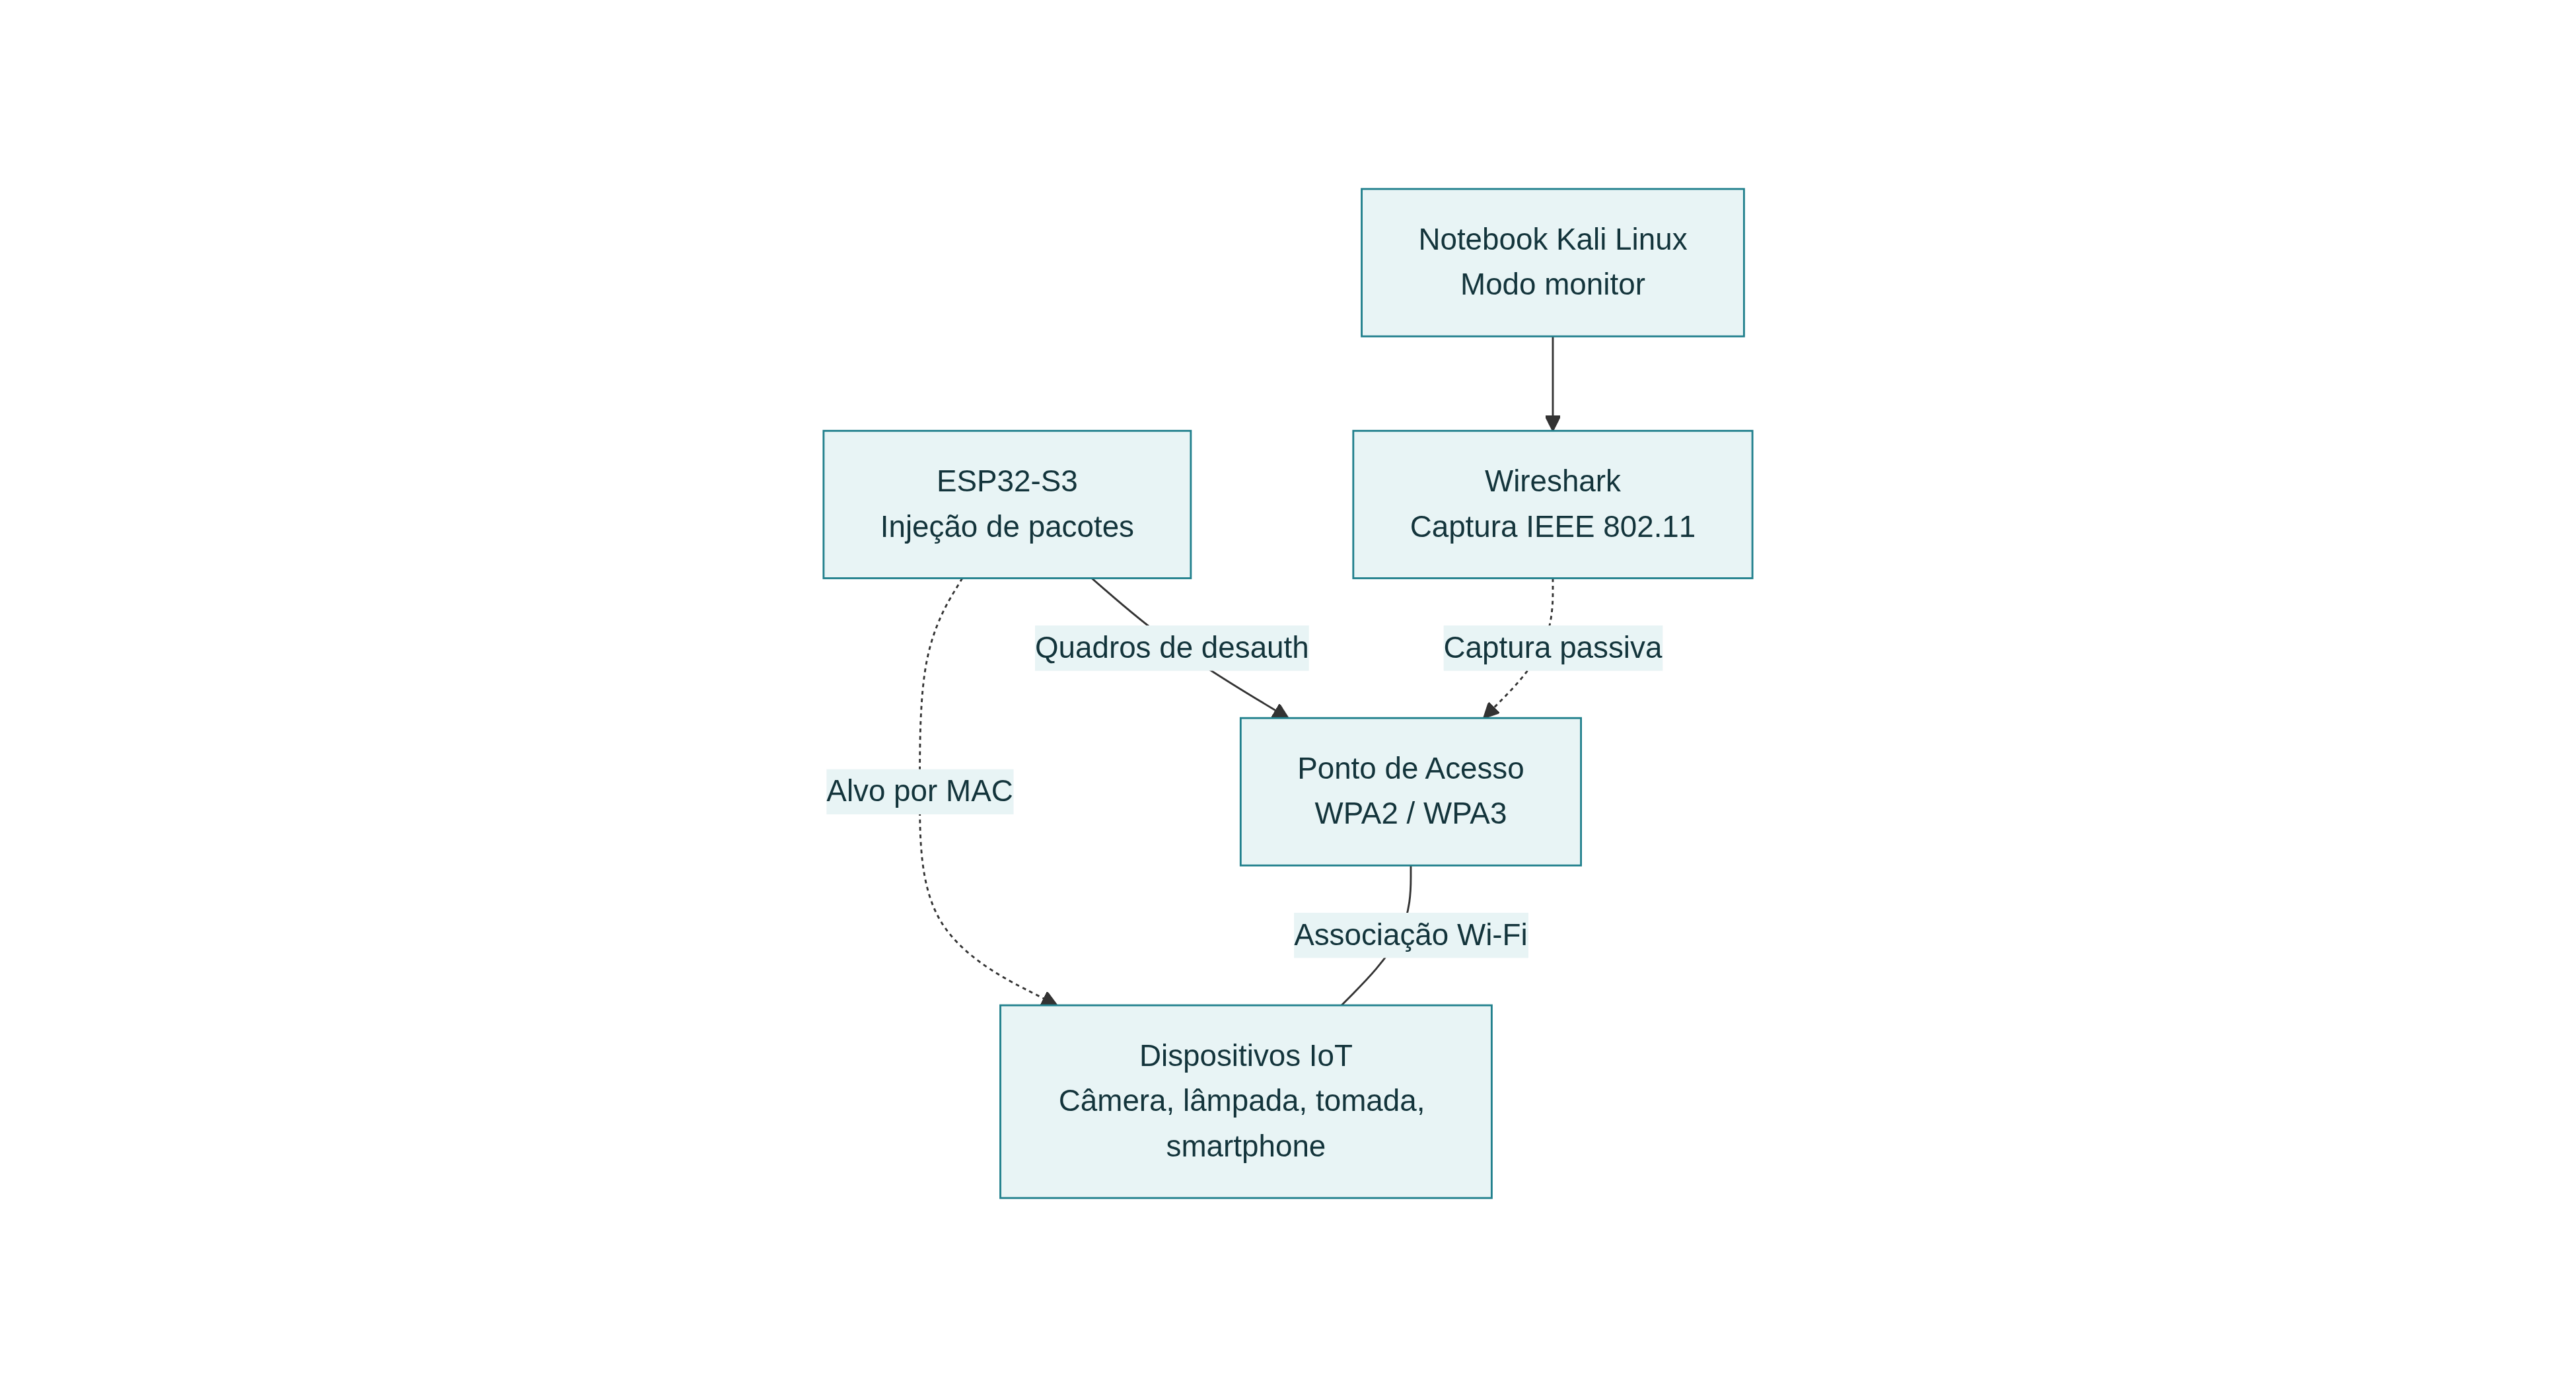
\includegraphics[
        width=0.88\textwidth,
        height=0.60\textheight,
        keepaspectratio
    ]{diagrama_blocos.jpg}
    \legend{Fonte: elaborado pelo autor (2026).}
\end{figure}

Como mostra a Figura~\ref{fig:diagrama_blocos}, a arquitetura teve quatro responsabilidades. O roteador e seu painel criaram a rede e definiram canal, segurança e PMF. O T-Embed CC1101 Plus, por meio do rádio Wi-Fi do ESP32-S3, transmitiu os quadros de desautenticação contra o dispositivo selecionado pelo endereço MAC. A câmera, a lâmpada e a tomada foram os dispositivos avaliados, e o \textit{smartphone} serviu como referência. Por fim, a estação de captura (Kali Linux, adaptador AR9271 em modo monitor) apenas registrou o tráfego e executou o \textit{ping}, sem participar da geração do ataque.

\section{Fluxograma do procedimento experimental}
\label{sec:atividades_experimento}

A Figura~\ref{fig:fluxograma_experimento} apresenta a sequência efetivamente seguida em cada ensaio, desde a configuração do ponto de acesso até a análise dos arquivos.

\begin{figure}[htbp]
\centering
\caption{Fluxograma do procedimento experimental}
\label{fig:fluxograma_experimento}
\begin{tikzpicture}[font=\normalsize, >=Stealth, node distance=5mm,
  b/.style={draw, rounded corners, fill=blue!7, text width=58mm, align=center, minimum height=11mm},
  d/.style={draw, diamond, aspect=2.2, fill=orange!14, text width=30mm, align=center, inner sep=1pt}]
\node[b] (s1) {Configurar o roteador no cenário (WPA2 ou modo misto), canal 6};
\node[b, below=of s1] (s2) {Confirmar o dispositivo associado e responder a \textit{ping}};
\node[b, below=of s2] (s3) {Iniciar, pelo \textit{script} na Kali, captura (\textit{tcpdump}, modo monitor) e \textit{ping} ao IP do dispositivo};
\node[b, below=of s3] (s4) {Janela de referência sem ataque};
\node[b, below=of s4] (s5) {Disparar a desautenticação no Bruce (ESP32-S3) contra o MAC do dispositivo};
\node[b, below=of s5] (s6) {Encerrar o ataque e observar a recuperação};
\node[b, below=of s6] (s7) {Encerrar captura e \textit{ping}; restabelecer o estado inicial (reinício da câmera ou espera)};
\node[d, below=7mm of s7] (q1) {Repetições do dispositivo concluídas?};
\node[d, below=9mm of q1] (q2) {Todos os dispositivos e cenários concluídos?};
\node[b, below=7mm of q2, fill=green!12] (s8) {Transferir os arquivos e analisar com \textit{tshark} e \textit{script} dos \textit{logs} de \textit{ping}};
\foreach \a/\b in {s1/s2,s2/s3,s3/s4,s4/s5,s5/s6,s6/s7,s7/q1} \draw[->] (\a) -- (\b);
\draw[->] (q1) -- node[right] {sim} (q2);
\draw[->] (q2) -- node[right] {sim} (s8);
\draw[->] (q1.east) -- node[above, pos=0.3] {não} ++(14mm,0) |- (s2.east);
\draw[->] (q2.west) -- node[above, pos=0.3] {não} ++(-14mm,0) |- (s1.west);
\end{tikzpicture}
\legend{Fonte: elaborado pelo autor (2026). No ensaio piloto, a captura foi feita pelo Wireshark, sem \textit{ping}.}
\end{figure}

Na Figura~\ref{fig:fluxograma_experimento}, a captura e o \textit{ping} foram iniciados juntos, antes do ataque, para registrar uma janela de referência; o ataque foi disparado manualmente no menu Wi-Fi do Bruce; e, ao final, o estado inicial do dispositivo foi restabelecido antes da repetição seguinte. Na câmera, esse restabelecimento exigiu reinício manual, porque ela não se reassociou sozinha. O protocolo completo, passo a passo, é detalhado no Apêndice~\ref{sec:protocolo}.

\section{Cadeia de processamento dos dados}
\label{sec:dados_captura}

Cada ensaio gerou um par de arquivos com o mesmo identificador, no formato \texttt{DISPOSITIVO\_CENÁRIO\_Rnn} (por exemplo, \texttt{LAMP\_WPA2\_R01.pcapng} e \texttt{LAMP\_WPA2\_R01\_ping.txt}). Ambos foram produzidos na máquina virtual Kali por um \textit{script} auxiliar, que, a partir do nome do ensaio, do IP do dispositivo e do canal, iniciava em paralelo o \textit{tcpdump} na interface em modo monitor e o \textit{ping} ao dispositivo, e os encerrava ao final. Os arquivos foram então transferidos para o computador hospedeiro, onde foi feita toda a análise. A Figura~\ref{fig:estrutura_evidencias} resume essa cadeia.

\begin{figure}[htb]
\centering
\caption{Cadeia de processamento das evidências de cada ensaio}
\label{fig:estrutura_evidencias}
\resizebox{\textwidth}{!}{%
\begin{tikzpicture}[font=\small, >=Stealth,
  e/.style={draw, rounded corners, minimum width=40mm, minimum height=15mm, align=center}]
\node[e, fill=blue!12] (exec) at (0,0) {\textit{Script} na Kali\\(nome, IP, canal 6)};
\node[e, fill=green!12] (pcap) at (5.5,1.3) {\texttt{.pcapng}\\(\textit{tcpdump}, Radiotap)};
\node[e, fill=green!12] (ping) at (5.5,-1.3) {\texttt{\_ping.txt}\\(\textit{ping} com marcas\\de tempo Unix)};
\node[e, fill=orange!16] (ts) at (11.5,1.3) {\textit{tshark}: deauth por MAC,\\autenticação/associação,\\RSN (AKM, MFPC/MFPR)};
\node[e, fill=orange!16] (py) at (11.5,-1.3) {\textit{Script} Python: intervalos\\sem resposta $>$2~s,\\maior queda contínua};
\node[e, fill=gray!14] (tab) at (17,0) {Tabelas e registro por\\execução do Cap.~5};
\draw[->] (exec) -- (pcap); \draw[->] (exec) -- (ping);
\draw[->] (pcap) -- (ts); \draw[->] (ping) -- (py);
\draw[->] (ts) -- (tab); \draw[->] (py) -- (tab);
\end{tikzpicture}}
\legend{Fonte: elaborado pelo autor (2026).}
\end{figure}

Como indica a Figura~\ref{fig:estrutura_evidencias}, as duas vertentes foram processadas separadamente:

\begin{itemize}
    \item \textbf{Das capturas (\textit{tshark})} vieram: o número de quadros de desautenticação com o endereço do dispositivo como origem ou destino (filtro de subtipo 12); os quadros de autenticação e associação, usados para identificar perda de associação; e os campos do elemento RSN (AKM, MFPC e MFPR) dos \textit{beacons} e dos \textit{Association Requests}.
    \item \textbf{Dos \textit{logs} de \textit{ping}} vieram: o tempo acumulado sem resposta (soma dos intervalos entre respostas consecutivas superiores a 2~s), a fração desse tempo sobre a duração do \textit{log} e a maior queda contínua.
\end{itemize}

A sincronização entre as duas fontes decorre de ambas terem sido geradas pela mesma máquina, com o mesmo relógio: o \textit{ping} foi executado com marcas de tempo absolutas (época Unix) em cada resposta, e o arquivo de captura registra o instante absoluto de cada quadro. Nos arquivos verificados (\texttt{LAMP\_WPA2\_R01}, \texttt{TOMADA\_WPA2\_R01} e \texttt{CAM\_WPA3\_R01}), a primeira resposta de \textit{ping} ocorreu até 0,5~s após o primeiro quadro capturado, o que confirma o início conjunto. Não houve sincronização com relógio externo, de modo que a comparação é válida entre as duas fontes de um mesmo ensaio, e não com horários de outros equipamentos. Os \textit{logs} contêm respostas marcadas como duplicadas (\texttt{DUP!}), acompanhadas do aviso \textit{wrong data byte} e de tempo \texttt{0.000~ms}; essas respostas, inclusive a primeira de cada série, que o \textit{ping} não marca como duplicada, foram descartadas no cálculo, feito pelo \textit{script} \texttt{src/analisa\_ping.py}, por corresponderem a eco de conteúdo corrompido e não a uma resposta válida, conforme a definição da métrica de perda de pacotes na Seção~\ref{subsec:dicionario_metricas}.

\section{Registro fotográfico do ambiente montado}
\label{sec:registro_fotografico}

Esta seção apresenta o registro fotográfico dos principais equipamentos montados na bancada experimental: o ponto de acesso, a plataforma de ataque e dois dos dispositivos IoT avaliados (câmera IP e tomada inteligente).

A Figura~\ref{fig:foto_roteador} apresenta o roteador TP-Link EX1500 empregado
como ponto de acesso da rede de teste, responsável por disponibilizar a rede
Wi-Fi e pelas configurações de segurança WPA2 e modo misto.

\begin{figure}[htb]
    \centering
    \caption{Roteador TP-Link EX1500 utilizado como ponto de acesso}
    \label{fig:foto_roteador}
    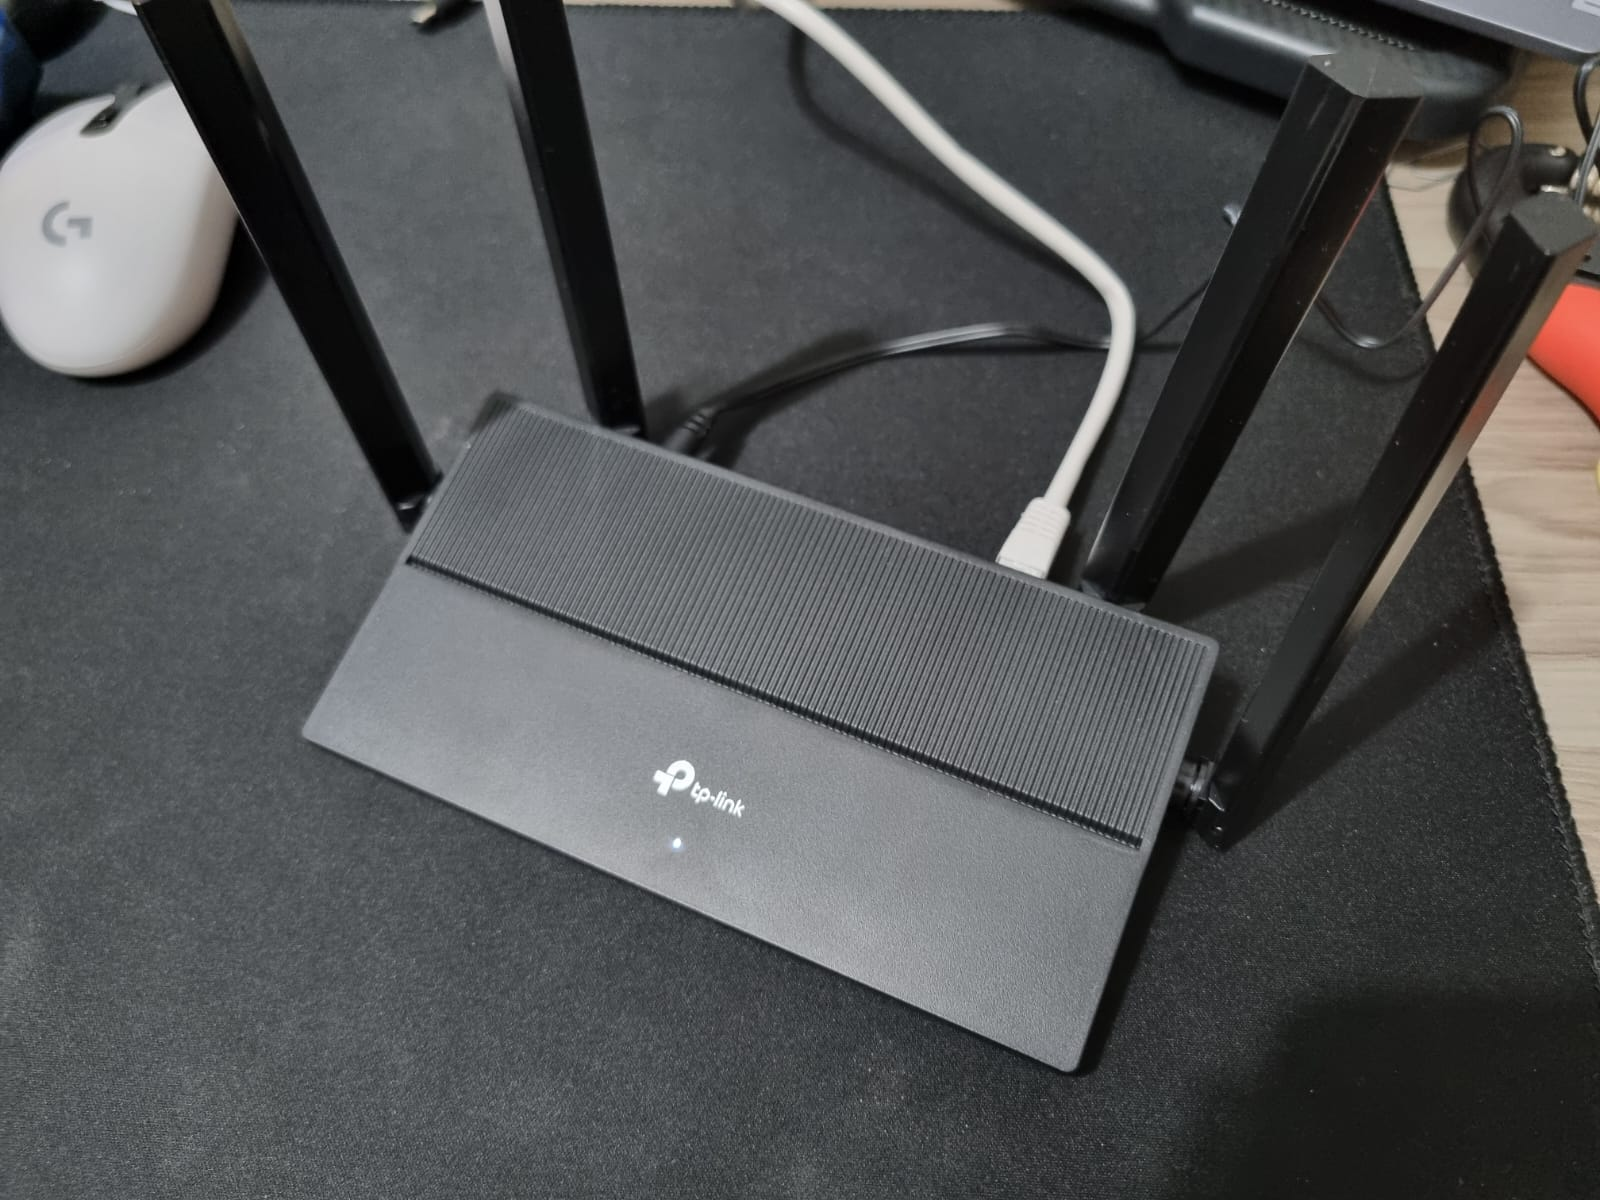
\includegraphics[width=0.72\textwidth,height=0.42\textheight,keepaspectratio]{foto_roteador.jpg}
    \legend{Fonte: elaborado pelo autor (2026).}
\end{figure}

A Figura~\ref{fig:foto_lilygo} apresenta a plataforma LILYGO T-Embed CC1101 Plus,
baseada em ESP32-S3 e executando o \textit{firmware} Bruce~1.16.1, utilizada como
plataforma de ataque. A tela exibe o menu de funções Wi-Fi do \textit{firmware}.

\begin{figure}[htb]
    \centering
    \caption{Plataforma LILYGO T-Embed CC1101 Plus com \textit{firmware} Bruce}
    \label{fig:foto_lilygo}
    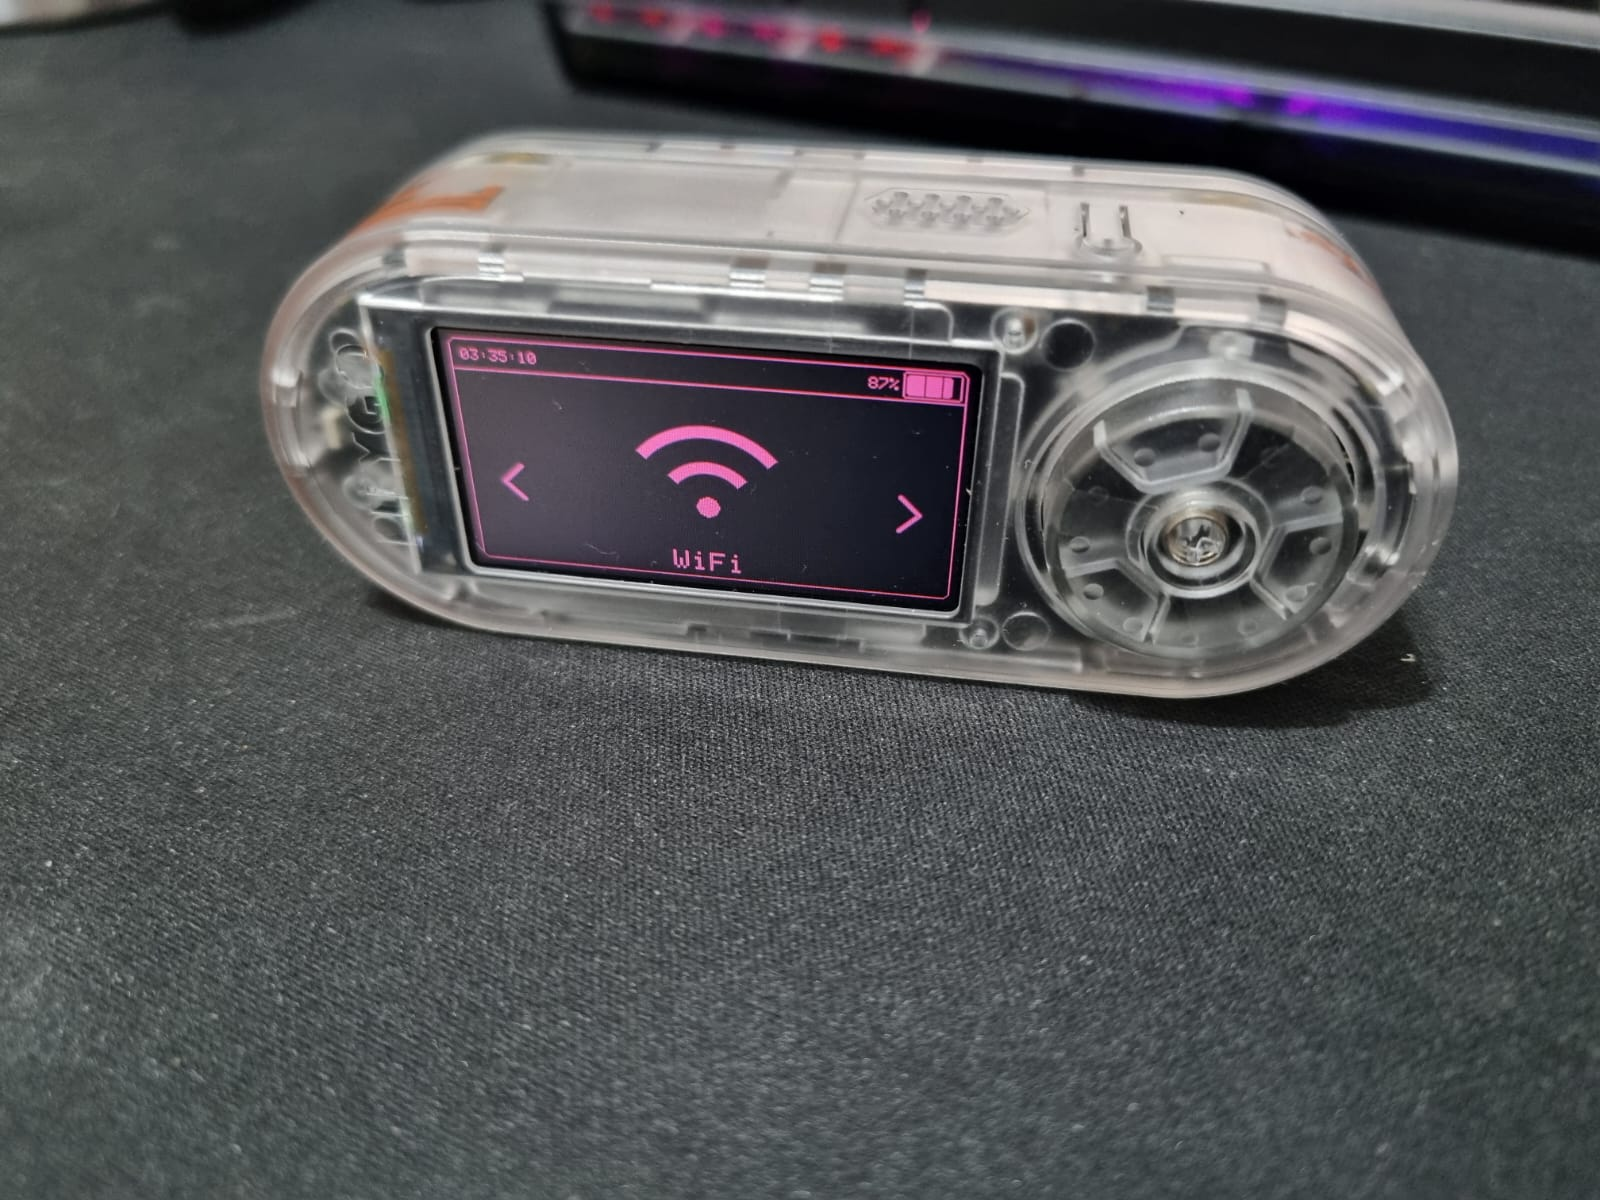
\includegraphics[width=0.72\textwidth,height=0.42\textheight,keepaspectratio]{foto_lilygo.jpg}
    \legend{Fonte: elaborado pelo autor (2026).}
\end{figure}

A Figura~\ref{fig:foto_camera} apresenta a câmera IP Xiaomi (identificada
comercialmente como Mi 360 PTZ 2K), utilizada tanto no ensaio piloto quanto nos
ensaios do conjunto completo de dispositivos.

\begin{figure}[htb]
    \centering
    \caption{Câmera IP Xiaomi utilizada como dispositivo IoT avaliado}
    \label{fig:foto_camera}
    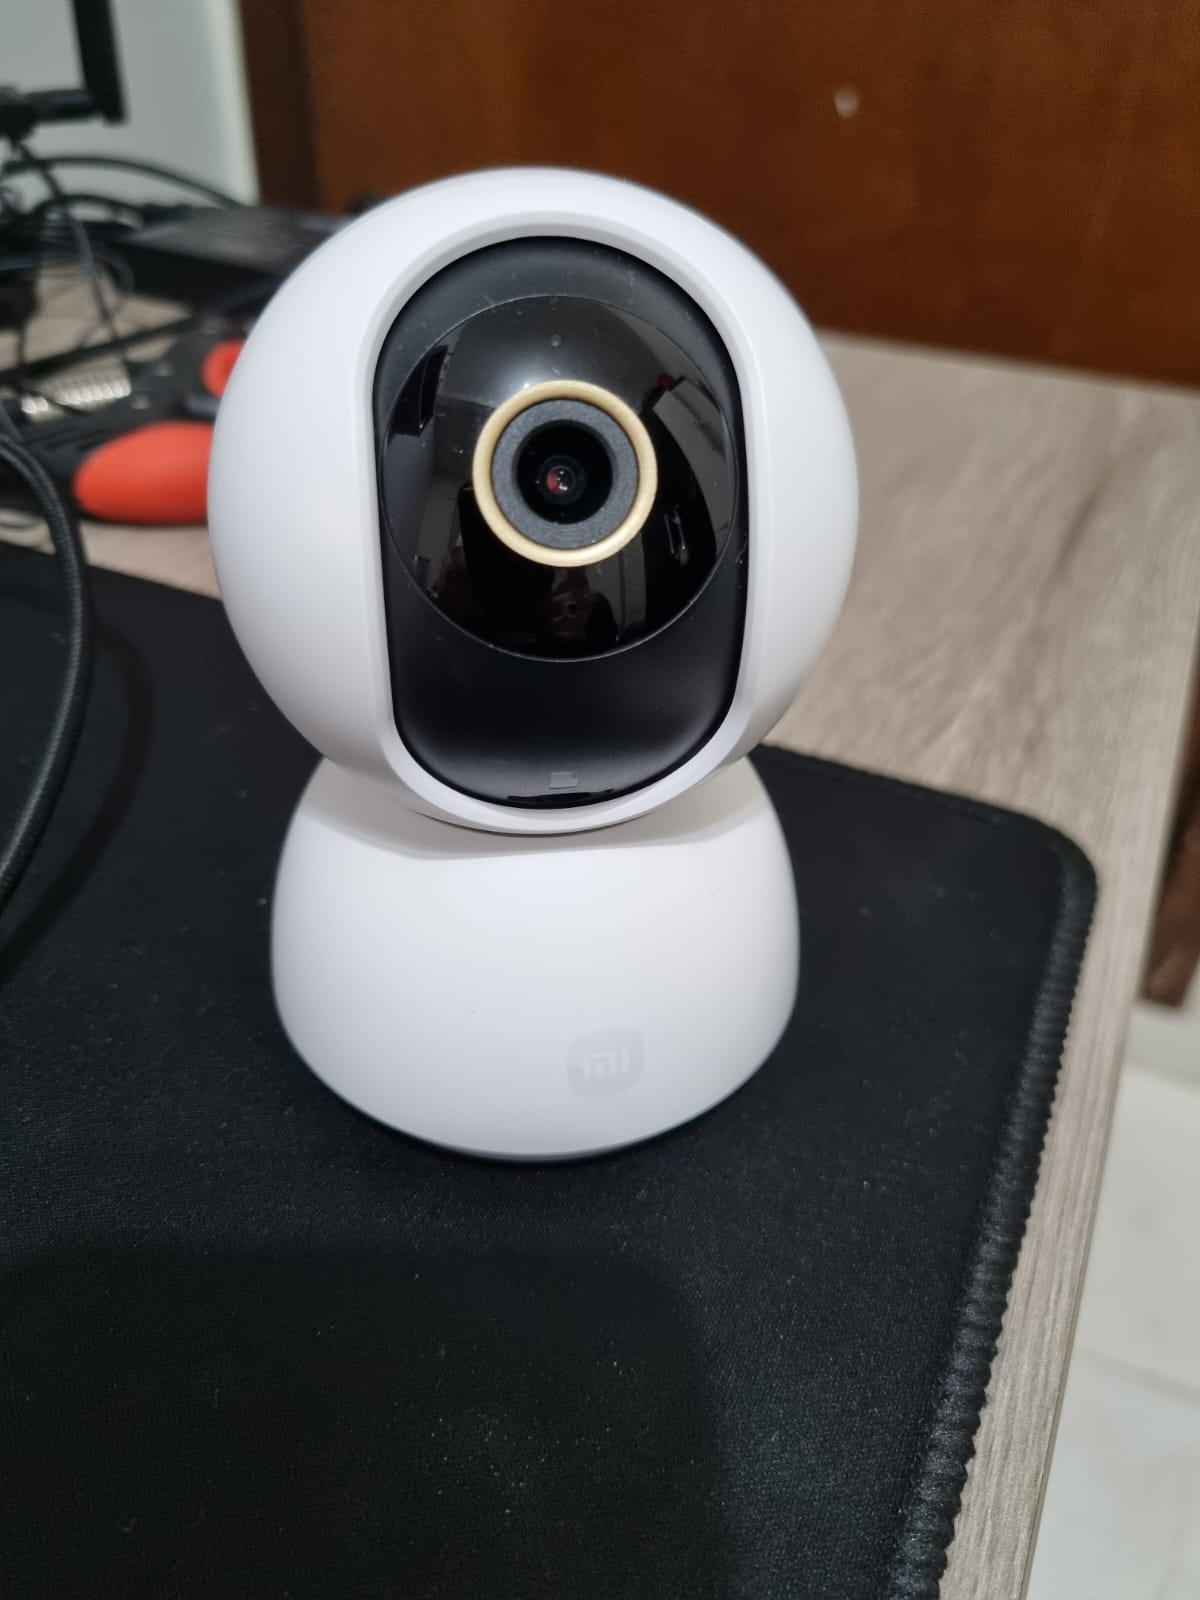
\includegraphics[width=0.60\textwidth,height=0.42\textheight,keepaspectratio]{foto_camera.jpg}
    \legend{Fonte: elaborado pelo autor (2026).}
\end{figure}

A Figura~\ref{fig:foto_tomada} apresenta a tomada inteligente, um dos
dispositivos IoT avaliados no experimento, conectada à rede de teste.

\begin{figure}[htb]
    \centering
    \caption{Tomada inteligente utilizada como dispositivo IoT avaliado}
    \label{fig:foto_tomada}
    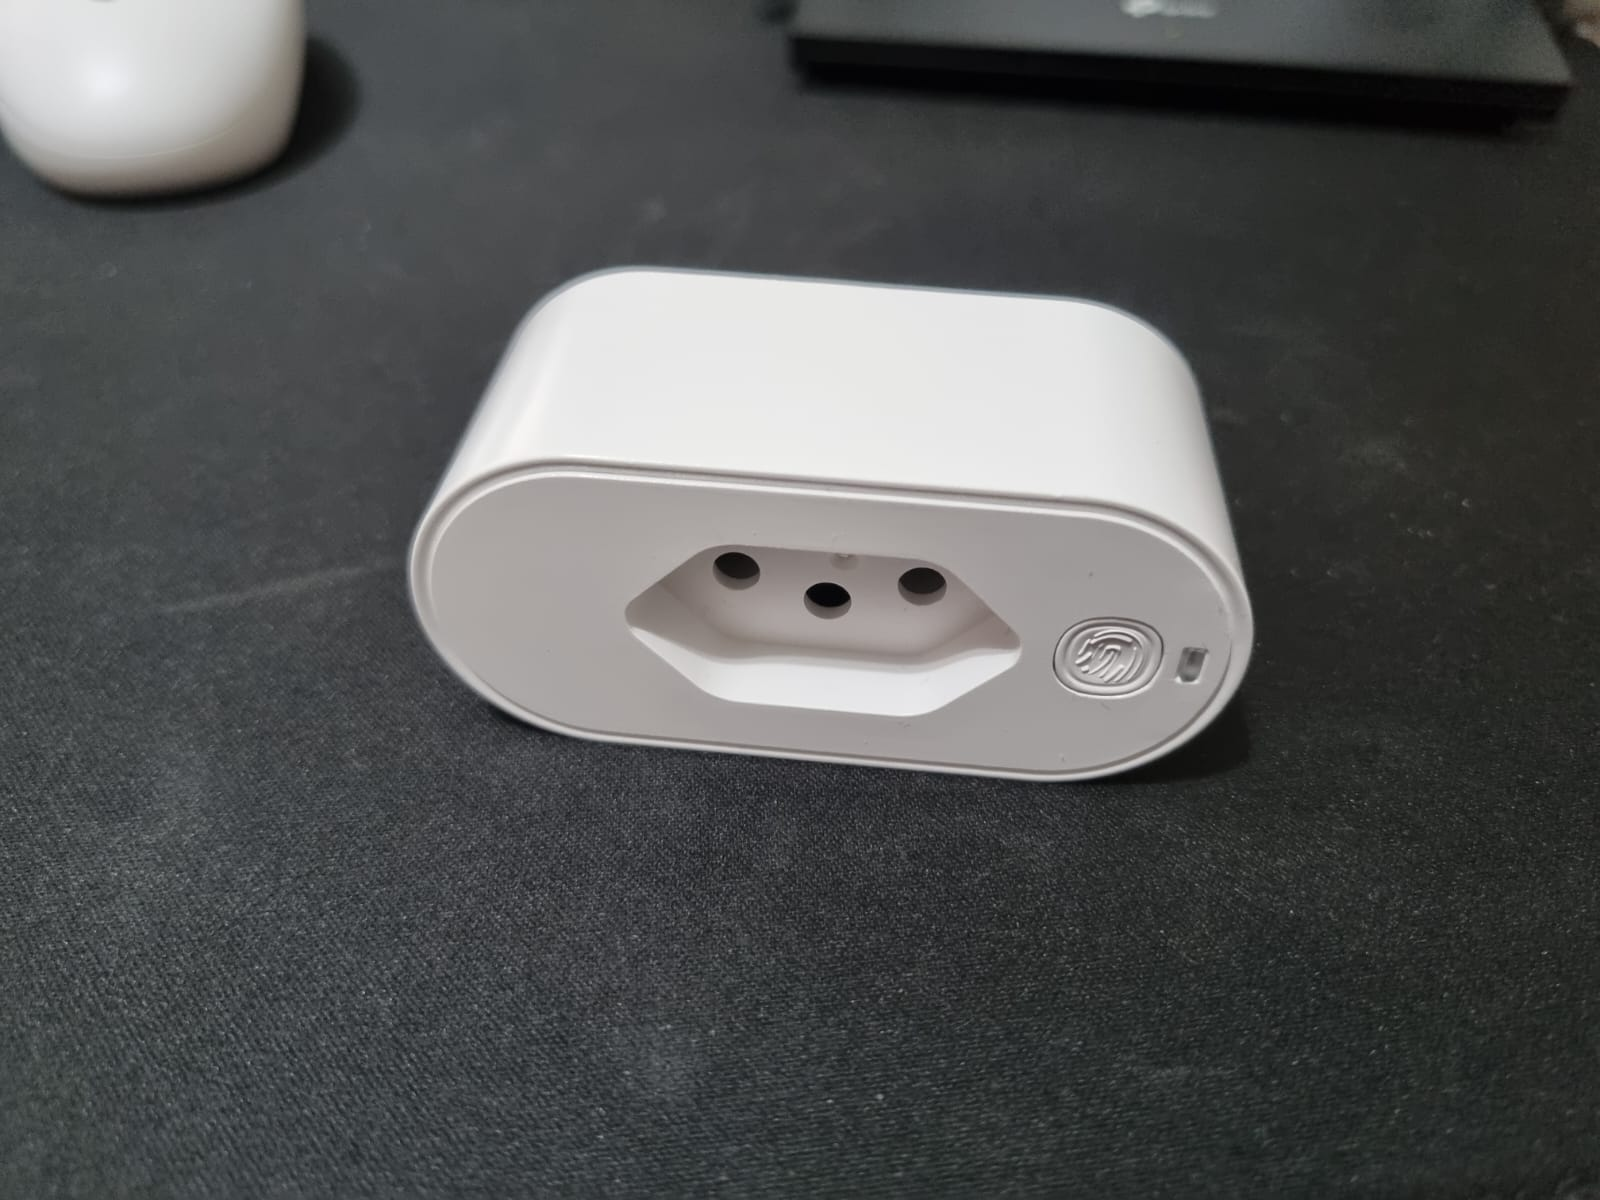
\includegraphics[width=0.72\textwidth,height=0.42\textheight,keepaspectratio]{foto_tomada.jpg}
    \legend{Fonte: elaborado pelo autor (2026).}
\end{figure}

\section{Critérios de validação aplicados}
\label{sec:criterios_validacao}

O ambiente foi considerado validado com base em evidências técnicas. Cada configuração de segurança foi validada pelo painel do roteador e pelos \textit{beacons} capturados, que registraram AKM e bits de PMF coerentes com a configuração pretendida. A associação de cada dispositivo foi validada pela resposta a \textit{ping} no início do ensaio. A captura foi considerada válida quando o adaptador gravou quadros IEEE~802.11 do canal 6 em arquivo \texttt{.pcapng} legível, o que ocorreu em todos os ensaios. A execução do ataque foi validada pela presença, na captura, de quadros de desautenticação com o endereço do dispositivo como origem ou destino; a execução \texttt{PHONE\_WPA3\_R02}, sem quadros de desautenticação direcionados ao \textit{smartphone}, não atendeu a esse critério. Além disso, uma execução foi considerada válida quando houve linha de base, isto é, respostas normais ao \textit{ping} antes do primeiro quadro de desautenticação direcionado ao dispositivo; nas execuções válidas, essa linha de base variou de cerca de 8,5~s a 105~s (Tabela~\ref{tab:registro-execucoes}). As execuções \texttt{CAM\_WPA2\_R05} e \texttt{CAM\_WPA2\_R06} não atenderam a esse critério e foram invalidadas: os quadros de desautenticação direcionados à câmera começaram aos 2,6~s e aos 0,5~s da captura, respectivamente, sem linha de base com \textit{ping} normal.

\section{Limitações do ambiente}
\label{sec:limitacoes_ambiente}

Os resultados ficam delimitados aos equipamentos, versões, configurações e cenários efetivamente utilizados; a amostra foi não probabilística e intencional, e os resultados não devem ser generalizados para todos os roteadores, dispositivos IoT ou redes IEEE~802.11.

No ambiente executado, as principais limitações foram: o número de repetições inferior ao planejado para a câmera e para o modo misto; a ausência de condições de WPA2 com PMF e de WPA3 exclusivo; a operação restrita a 2,4~GHz da plataforma de ataque e do adaptador de captura; o agrupamento dos ensaios por cenário, que faz o horário variar junto com a configuração; a distância entre os equipamentos, que não foi medida, e a potência de transmissão e a carga da rede, registradas mas não controladas como variáveis do ensaio (Quadro~\ref{quad:condicoes}); e a sincronização das fontes apenas pelo relógio da máquina virtual. Interferências de radiofrequência de redes vizinhas e atualizações automáticas dos dispositivos não foram controladas.
